\chapter{Fluxo de utilização}

Este capítulo apresenta as funcionalidades disponíveis para a operação do simulador através da interface gráfica, tais quais:

\begin{itemize}
\setlength{\itemsep}{1pt}
\setlength{\parskip}{0pt}
\setlength{\parsep}{0pt}
\item Seleção de cenário
\item Seleção de modelo de VANT
\item Configuração de cenário
\item Edição de configurações do VANT
\item Inicialização de simulação.
\end{itemize}
 
\section{Como inicializar o ambiente de simulação}

Tendo realizado o processo de instalação do simulador com exito, como descrito no capítulo anterior, pode-se iniciar o processo de desenvolvimento de controladores no ambiente de simulação ProVANT. Para iniciar a interface gráfica do usuário abra um novo terminal e digite o seguinte comando:

\begin{bashcode}
$ provant_gui
\end{bashcode}

A interface gráfica de acesso ao simulador será então incializada e aparecerá a janela principal, como ilustrado na Figura \ref{1}.

\begin{figure*}[!ht]
	\centering
	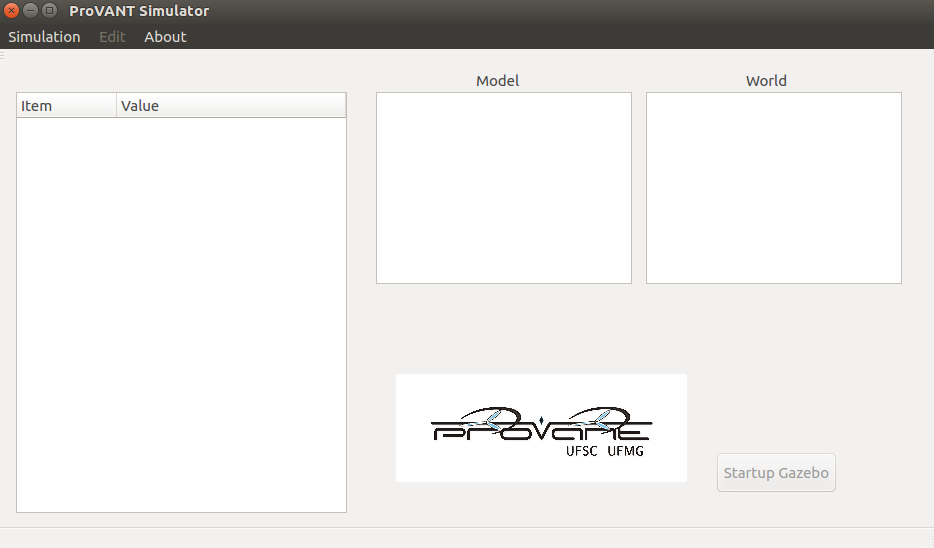
\includegraphics[width=0.8\columnwidth]{figuras/1.png}
	\caption{Janela inicial.}
	\label{1}
\end{figure*}

\section{Seleção de cenário}

Tendo inicializado a interface gráfica do ambiente de simulação, é necessário que o usuário selecione um cenário de simulação. Isso pode ser realizado de duas maneiras diferentes, ambas através da utilização da opção "Simulation", presente no menu superior da interface gráfica, ilustrado na figura \ref{2}: 

\begin{figure*}[!ht]
	\centering
	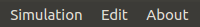
\includegraphics[width=100pt]{figuras/2.png}
	\caption{Menu superior.}
	\label{2}
\end{figure*}

\begin{itemize}
	\item[(i)] Ao clicar em "New", é possível abrir um cenário template com extensão ".tpl".
	
	Um cenário template é um uma configuração de cenário que serve de molde para a criação de outros cenários. Ele não pode ser editado, necessita da adição de um modelo de um VANT e deve ser salvo antes da simulação com o formato ".world"
	 
	\item[(ii)] Ao clicar em "Open", é possível abrir um cenário já existente (arquivo com extensão ".world").  
	
	\item[(iii)] Ao clicar em "About", é possível conferir informações gerais do simulador ProVANT .  
\end{itemize}
  
Ainda no menu "Simulation", é possível salvar um cenário com outro nome no formato ".world", clicando em ("Save"), e também finalizar o ambiente de simulação, clicando em ("Exit").

\section{Seleção do VANT}

Através da opção "Edit", no menu superior, é possível selecionar modelo de VANT a ser utilizado na simulação. Atenção: nessa versão do ambiente de simulação, é possível apenas a adição de de um único VANT na mesma instância de simulação.

\section{Janela de configuração da simulação}

Tendo escolhido o VANT e o cenário de simulação, suas imagens a imagem ilustrativa do cenário aparecerá na interface e portanto é possível verificar se foram selecionados corretamente, como mostra a Figura \ref{tela_inicial.jpg}, através dos itens (2) e (3), respectivamente. 
% É possível também visualizar parâmetros e configurações de itens relacionados aos mesmos, como gravidade, posição e orientação iniciais, etc. 

\begin{figure*}[!ht]
	\centering
	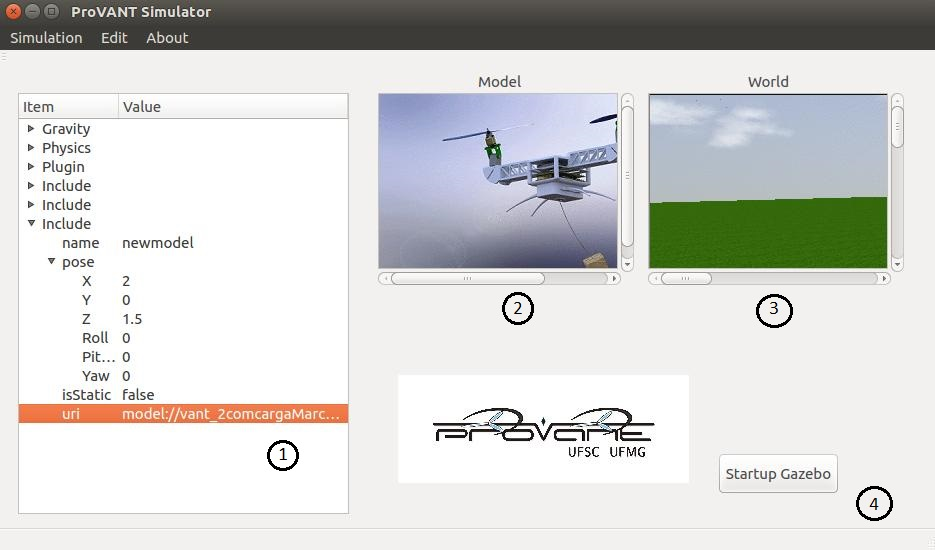
\includegraphics[width=500pt]{figuras/tela_inicial.jpg}
	\caption{Janela de configuração da simulação.}
	\label{tela_inicial.jpg}
\end{figure*}

Ainda com relação à Figura \ref{tela_inicial.jpg}, o item (1) corresponde à uma árvore de informações e configurações do VANT e do cenário de simulação. Através de duplo clique em cima do campo desejado é possível realizar configurações. Os campos dessa arvore são:

\begin{itemize}
	\item Gravity: vetor de aceleração da gravidade com relação ao referencial do mundo em $m/s^2$; 
	\item Physics: motor físico física utilizada para realizar simulação. As opções possíveis são:
	\begin{itemize}
		\setlength{\itemsep}{1pt}
		\setlength{\parskip}{0pt}
		\setlength{\parsep}{0pt}
		\item ode (propositório de criação: dinâmica simplificada para robôs)
		\item bullet (propositório de criação: jogos)
		\item dart: (propositório de criação: computação gráfica e controle de robôs)
		\item simbody (propositório de criação: plicações biomecânicas)
	\end{itemize}
	\item name: Nome do modelo do VANT no simulador Gazebo.;
	\item pose: Posição (x,y,z) e orientação (roll,pitch,yaw) iniciais do VANT, em $m$ e $rad$, respectivamente.   
\end{itemize}

\noindent Através do duplo clique no campo uri, uma nova janela se abrirá, na qual é possível visualizar e realizar configurações no modelo, controlador, atuadores e sensores. Mais detalhes sobre está janela são apresentados na próxima seção. O item (4) permite a inicialização da simulação com as configurações, modelo e cenário selecionados pelo usuário na interface gráfica.

%Os itens número 2 e 3 correspondem, respectivamente, as imagens que ilustram o VANT e o cenário selecionados para simulação.

\section{Janela de visualização e configuração dos parâmetros do modelo, estratégia de controle e instrumentação}
\label{SecEstCtrl}

Como mencionado, através de duplo clique no campo uri uma nova janela de configurações será aberta, como mostra a Figura \ref{4}. Através das quatro abas disponíveis: Parameters, Controller, Sensors e Actuators; é possível gerenciar as configurações do modelo, estratégia de controle e instrumentação utilizados para simulação. A janela é inicializada com a aba Parameters selecionada. Esta aba permite a visualização dos parâmetros do modelo do VANT utilizado na simulação.

\begin{figure*}[!ht]
	\centering
	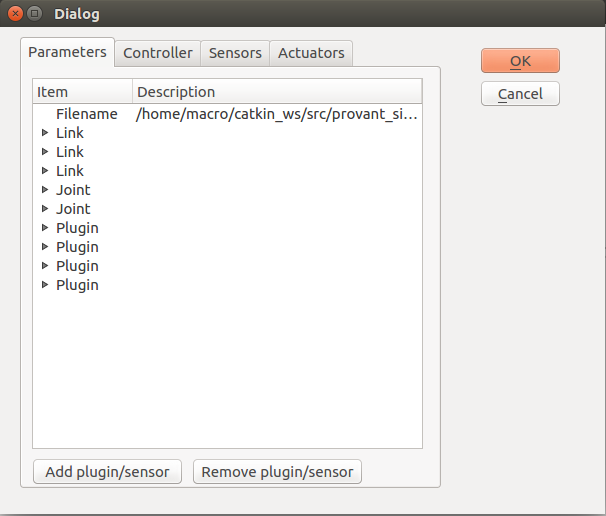
\includegraphics[width=250pt]{figuras/4.png}
	\caption{Aba para visualização dos parâmetros do modelo do VANT.}
	\label{4}
\end{figure*}

A Figura \ref{5} mostra a aba "Controller". Nela é possível criar uma nova estratégia de controle, utilizando o item (2), selecionar uma existente, através do item (3) ou compilá-las, item (4). A estratégia de controle selecionada para ser utilizada na simulação é mostrada no item (1). Mais detalhes sobre esses itens são descritos a seguir.

\begin{figure*}[!ht]
	\centering
	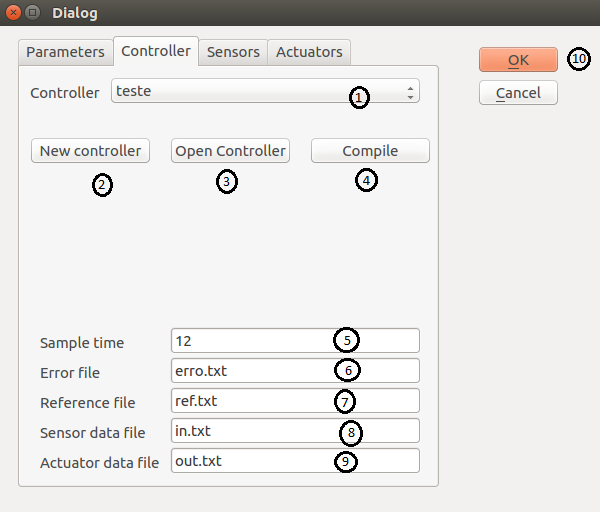
\includegraphics[width=250pt]{figuras/5_2.png}
	\caption{Aba para seleção e configuração da estratégia de controle.}
	\label{5}
\end{figure*}

\subsubsection{Criando uma nova estratégia de controle}

Para criar uma nova estratégia de controle, deve-se clicar no botão "New controller" $~$ item (2), e uma nova janela será mostrada (Figura \ref{9}). Nesta janela, o usuário deve inserir o nome da nova estratégia de controle (mais detalhes sobre a criação de uma nova estratégia de controle são apresentados no Capítulo \ref{controle}).

\begin{figure*}[!ht]
	\centering
	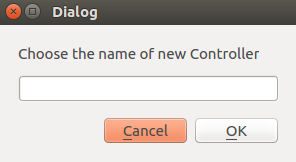
\includegraphics[width=100pt]{figuras/9.png}
	\caption{Criando uma nova estratégia de controle.}
	\label{9}
\end{figure*}

\subsubsection{Modificando uma estratégia de controle já existente}

Para modificar uma estratégia de controle já existente, o usuário deve selecionar o nome da estrategia de controle entre várias listadas na caixa de listagem item (1) e clicar na botão "Open controller" item (3). Após escolher a estratégia, o gerenciador de arquivos Nautilus será aberto no diretório com todos os arquivos e diretórios associados ao controlador, conforme mostra a Figura \ref{10}.

% (colocar uma figura com essa janela e citar ela).%

\begin{figure*}[!ht]
	\centering
	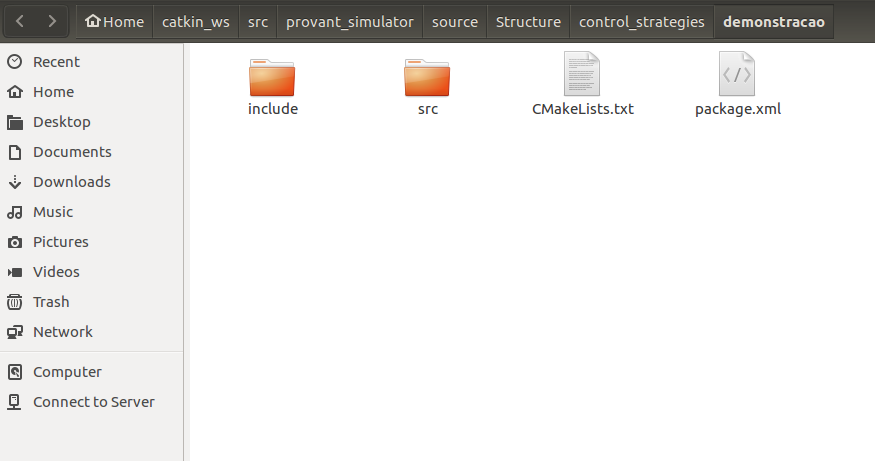
\includegraphics[width=300pt]{figuras/10.png}
	\caption{Diretório contendo arquivos e pastas associados à estratégia de controle a ser modificada.}
	\label{10}
\end{figure*}

\subsubsection{Compilando o controlador}

Para compilar o código associado à estratégia de controle selecionada, o usuário deve clicar no botão "Compile" $~$ item (4). \textbf{Esta etapa deve ser realizada sempre que haja modificações na estratégia de controle}. Caso ocorram erros durante a compilação, o relatório de saída do compilador será mostrado em um arquivo de texto por meio do aplicativo gedit.

\subsubsection{Alterando configurações adicionais }

A aba ''Controller'' também permite a configuração de outros parâmetros associados à simulação. O campo ''Sample time'', item (5), permite a configuração do perído de amostragem em milissegundos. Já os demais campos, ''Error file'', item (6), ''Reference data file'', item (7), ''Sensor file'', item (8) e ''Actuator data file'', item (9) determinam o nome dos arquivos de texto onde serão registrados os valores do erro dos estados, trajetória desejada, dados dos sensores e sinais de controle, respectivamente. Estes arquivos podem ser carregados diretamente no MATLAB. Tais arquivos estarão disponíveis no diretório: 

\begin{bashcode}
$HOME/catkin_ws/srcProVANT-Simulator/source/Structure/Matlab
\end{bashcode}

\subsection{Selecionando a instrumentação disponível}
\label{sensoresatuadores}

As abas Sensors e Actuators, ilustradas na Figura \ref{6}, listam, respectivamente, os nomes dos tópicos dos sensores e atuadores que o controlador terá acesso durante a simulação \textbf{de acordo a ordem apresentada}. Tais tópicos são configurados durante a configuração dos plugins, sendo melhor detalhados na seção \ref{plugins}. 

Conforme necessário, o usuário deve adicionar, remover e editar os intrumentos (atuadores/sensores) disponíveis na lista. Para adicionar novos instrumentos basta selecionar o botão ''Add'' e clicar duas vezes no nome do instrumento desejado. Para removê-los, basta selecionar o instrumento e pressionar o botão ''Remove''. 

\begin{figure}
	\hfill
	\subfloat{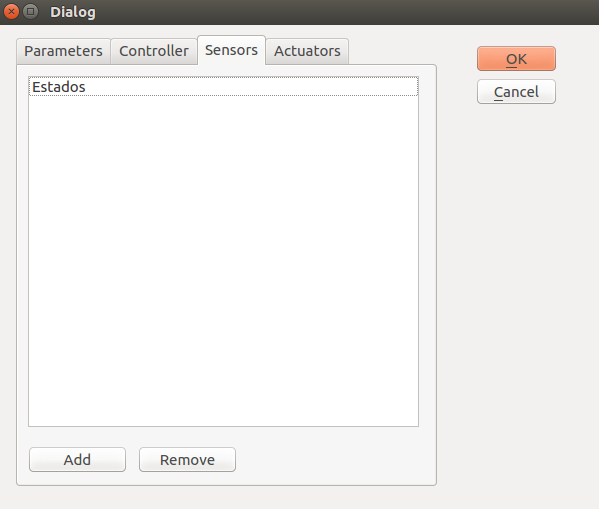
\includegraphics[width=230pt]{figuras/6.png}}
	\hfill
	\subfloat{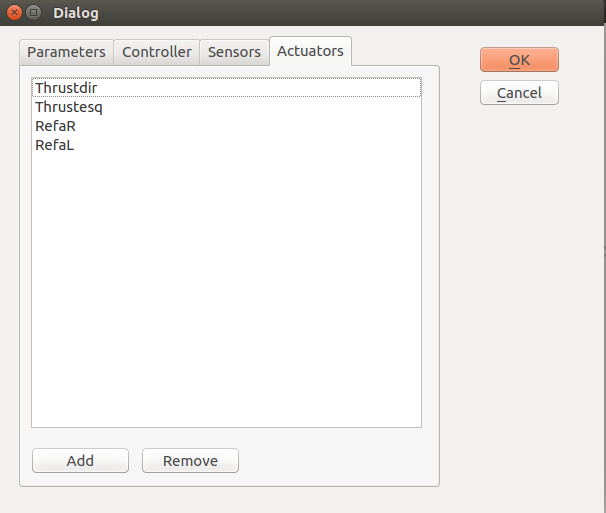
\includegraphics[width=230pt]{figuras/7.png}}
	\hfill
	\caption{Abas para seleção da instrumentação disponível durante a simulação.}
	\label{6}
\end{figure}


\subsection{Inicializando a simulação}

Após realizar todas as configurações, o usuário deve pressionar o botão "OK" $~$ item (10). A janela de configuração da simulação (Figura \ref{tela_inicial.jpg}) será mostrada novamente. A simulação pode ser então inicializada com o modelo de VANT, cenário, estratégia de controle e instrumentação selecionados, através do botão "Startup Gazebo" $~$, item (4) da Figura \ref{tela_inicial.jpg}. O simulador Gazebo será inicializado, conforme mostrado na Figura \ref{12}. 



\begin{figure*}[!ht]
	\centering
	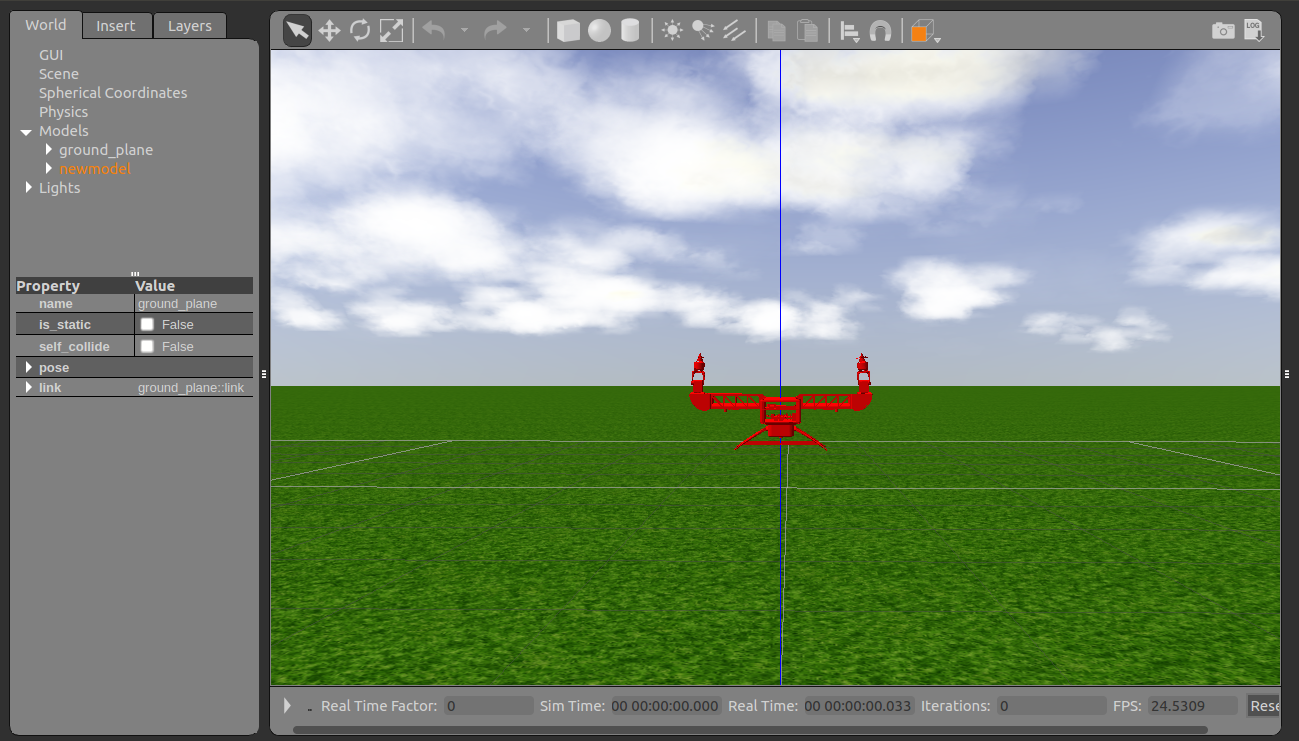
\includegraphics[width=400pt]{figuras/12.png}
	\caption{Janela inicial do simulador Gazebo.}
	\label{12}
\end{figure*}

Para dar início à simulação, o usuário deve pressionar o botão STEP. \textbf{O botão PLAY não deve ser utilizado}.